\chapter{Лекция 3. Строгий порядок. Замыкания. Основы теории графов}

% === Строгий порядок ===

\begin{defn}{Строгий порядок}{strict-order}
$M \neq \varnothing$,\; $f\colon M^2 \to \mathbb{B}$.

$f$ --- \textbf{строгий порядок} $\;\Leftrightarrow\;$
$f$ асимметрично и транзитивно.
\end{defn}

\textbf{Пример:} $\mathbb{R},\; <$.

\begin{task}{}{task-asym}
Доказать, что асимметричность $\Rightarrow$ арефлексивность.
\tcblower
\textbf{Решение.} Асимметричность: $\forall\, a, b\colon
f(a,b) = 1 \Rightarrow f(b,a) = 0$. Возьмём $b = a$: если бы нашлось $a$
с $f(a,a) = 1$, то по асимметричности (при $b = a$) получили бы
$f(a,a) = 0$ --- противоречие. Значит $\forall\, a\colon f(a,a) = 0$,
т.\,е. отношение арефлексивно. $\blacksquare$
\end{task}

% === Замыкания ===
\bigskip
\begin{defn}{Замыкание бинарного отношения}{closure}
$M \neq \varnothing$,\; $f\colon M^2 \to \mathbb{B}$,\;
$\tilde{f}\colon M^2 \to \mathbb{B}$.

\textbf{Замыкание} $f$ относительно свойства $(*)$ --- это $\tilde{f}$, т.\,ч.:
\begin{enumerate}
  \item $\tilde{f}$ согласовано с $f$
        (т.\,е. $\forall\, a,b\colon f(a,b)=1 \Rightarrow \tilde{f}(a,b)=1$);
  \item $\tilde{f}$ обладает свойством $(*)$;
  \item $\tilde{f}$ имеет минимальный носитель среди всех б.\,о.,
        удовлетворяющих 1) и 2) (минимальное количество рёбер).
\end{enumerate}
\end{defn}

\begin{defn}{Носитель функции}{support}
$f\colon A \to B$. \textbf{Носитель} $f$:
\[
  \operatorname{supp}(f) := \bigl\{\, a \in A \;\big|\; f(a) \neq 0 \,\bigr\}.
\]
\end{defn}

\textit{Замечание:} замыкать можно только <<вверх>> (добавлять рёбра).
Например, замыкание по арефлексивности невозможно --- нельзя стирать рёбра.

\medskip
\textbf{Примеры замыканий.}

\begin{enumerate}
  \item \textbf{Рефлексивное замыкание:}
        граф $a \to b \to c$ --- добавляем петли у каждой вершины.

  \item \textbf{Симметричное замыкание:}
        $a \to b$, $b \to c$ --- добавляем обратные рёбра
        ($b \to a$, $c \to b$).
\end{enumerate}

\textbf{NB:} после рефлексивного и симметричного замыканий может нарушиться
транзитивность: $a \to b$ и $b \to c$ есть, но $a \to c$ нет
(транзитивная дуга отсутствует).

% === Алгоритм Флойда--Уоршелла ===
\bigskip
\begin{algo}{Алгоритм Флойда--Уоршелла (построение транзитивного замыкания)}{floyd-warshall-closure}
\textbf{Вход:} матрица смежности $A_f$ б.\,о. $f$ (размер $n \times n$).

\textbf{Выход:} матрица транзитивного замыкания $\tilde{A}$.

\textbf{Шаг 1:} $\forall\, v \in V$: рассматриваем $v$ как <<промежуточную>> вершину.

\textbf{Шаг 2:} Для каждой пары $(i, j)$: если $a_{iv} = 1$ и $a_{vj} = 1$,
то полагаем $a_{ij} := 1$.

Повторяем для всех вершин $v$.

После дорисовывания графа получаем транзитивное замыкание.
\end{algo}

\exhead{Пример.} Граф $a \to b \to c \to d$. Проследим работу алгоритма
сразу в двух представлениях: на графе и на матрице смежности. Новые
(дорисованные на текущем шаге) рёбра --- зелёные, добавленные ранее ---
светло-фиолетовые; промежуточная вершина $v$ --- оранжевая. В матрицах
новые единицы выделены жирным.

\medskip
\noindent Исходный граф и его матрица ($v = a$ ничего не даёт: в $a$ нет
входящих рёбер):

\begin{center}
\begin{tabular}{cc}
\raisebox{-0.5\height}{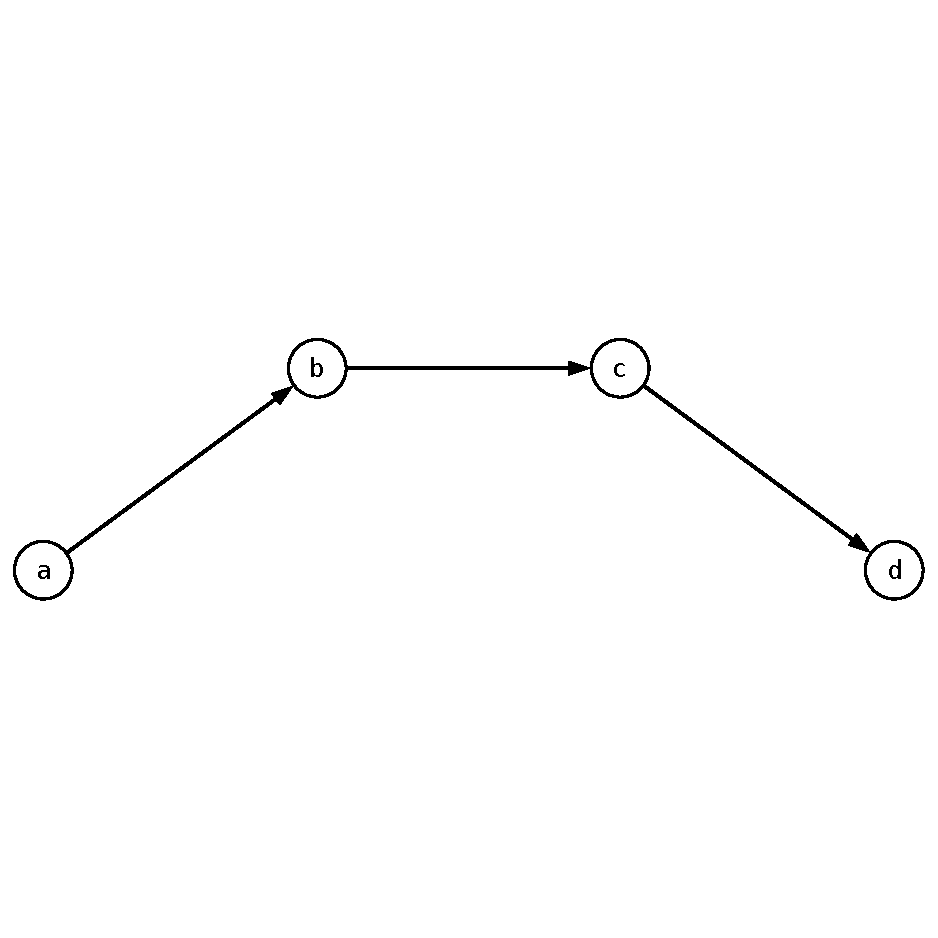
\includegraphics[width=0.42\textwidth]{figures/fw-step-0.pdf}} &
\renewcommand{\arraystretch}{1.25}
\begin{tabular}{|c||c|c|c|c|}
\hline
$f$ & \textbf{a} & \textbf{b} & \textbf{c} & \textbf{d} \\ \hline\hline
\textbf{a} & 0 & 1 & 0 & 0 \\ \hline
\textbf{b} & 0 & 0 & 1 & 0 \\ \hline
\textbf{c} & 0 & 0 & 0 & 1 \\ \hline
\textbf{d} & 0 & 0 & 0 & 0 \\ \hline
\end{tabular}
\end{tabular}
\end{center}

\noindent Промежуточная вершина $v = b$: есть $a \to b$ и $b \to c$,
поэтому дорисовываем $a \to c$ (т.\,е. $a_{ac} := 1$):

\begin{center}
\begin{tabular}{cc}
\raisebox{-0.5\height}{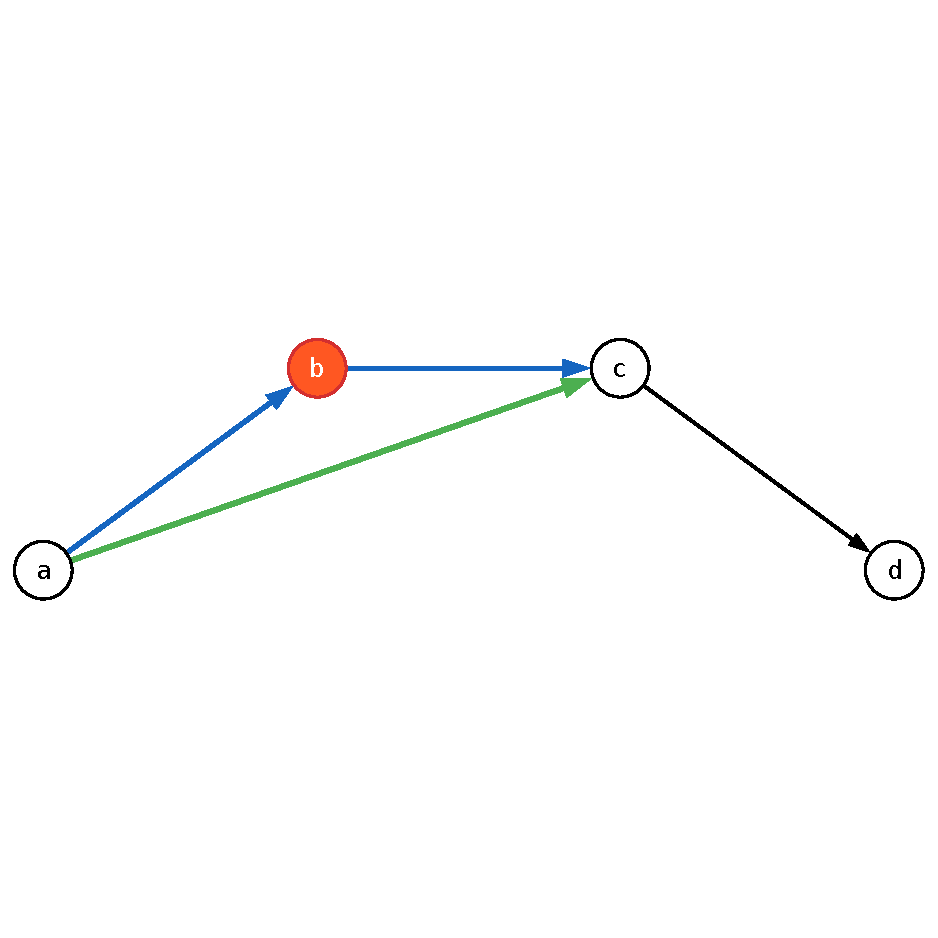
\includegraphics[width=0.42\textwidth]{figures/fw-step-1.pdf}} &
\renewcommand{\arraystretch}{1.25}
\begin{tabular}{|c||c|c|c|c|}
\hline
$f$ & \textbf{a} & \textbf{b} & \textbf{c} & \textbf{d} \\ \hline\hline
\textbf{a} & 0 & 1 & $\mathbf{1}$ & 0 \\ \hline
\textbf{b} & 0 & 0 & 1 & 0 \\ \hline
\textbf{c} & 0 & 0 & 0 & 1 \\ \hline
\textbf{d} & 0 & 0 & 0 & 0 \\ \hline
\end{tabular}
\end{tabular}
\end{center}

\noindent Промежуточная вершина $v = c$: в $c$ входят $a \to c$ и $b \to c$,
из $c$ выходит $c \to d$, поэтому дорисовываем $a \to d$ и $b \to d$:

\begin{center}
\begin{tabular}{cc}
\raisebox{-0.5\height}{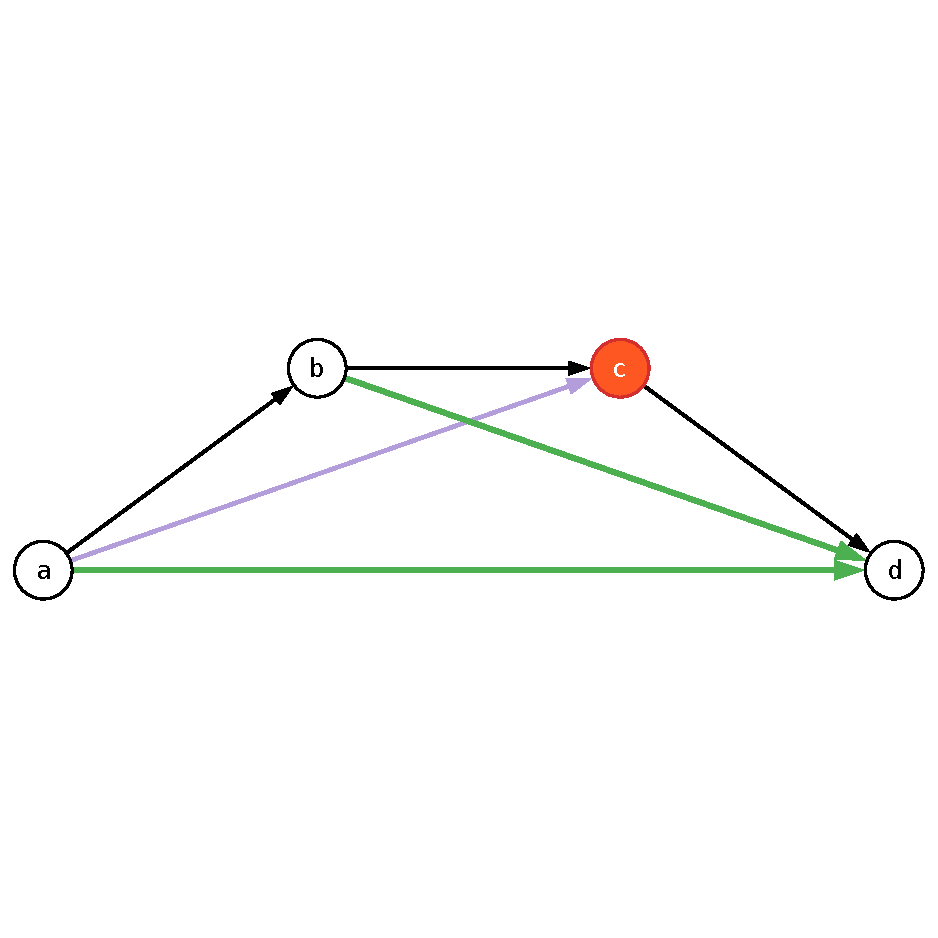
\includegraphics[width=0.42\textwidth]{figures/fw-step-2.pdf}} &
\renewcommand{\arraystretch}{1.25}
\begin{tabular}{|c||c|c|c|c|}
\hline
$f$ & \textbf{a} & \textbf{b} & \textbf{c} & \textbf{d} \\ \hline\hline
\textbf{a} & 0 & 1 & 1 & $\mathbf{1}$ \\ \hline
\textbf{b} & 0 & 0 & 1 & $\mathbf{1}$ \\ \hline
\textbf{c} & 0 & 0 & 0 & 1 \\ \hline
\textbf{d} & 0 & 0 & 0 & 0 \\ \hline
\end{tabular}
\end{tabular}
\end{center}

\noindent Промежуточная вершина $v = d$ ничего не добавляет (из $d$ нет
исходящих рёбер). Итог --- транзитивное замыкание
$\tilde f = \{a{\to}b,\; b{\to}c,\; c{\to}d,\; a{\to}c,\; a{\to}d,\; b{\to}d\}$:

\begin{center}
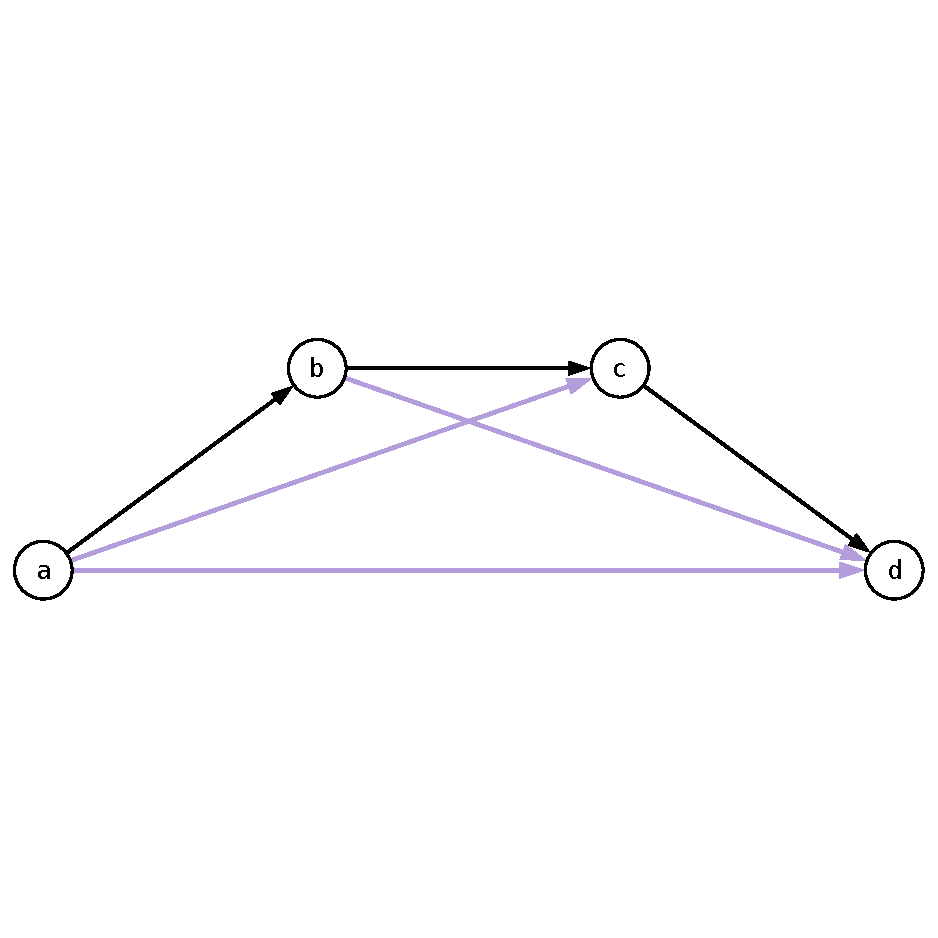
\includegraphics[width=0.42\textwidth]{figures/fw-step-3.pdf}
\end{center}

% === Основы теории графов ===
\bigskip
\subsection*{Основные понятия теории графов}

$G(V, E)$ --- \textbf{граф}, где $V$ --- множество вершин, $E$ --- множество рёбер.

Граф бывает:
\begin{itemize}
  \item \textbf{неориентированный} (ненаправленный) --- рёбра без направления;
  \item \textbf{ориентированный} (направленный) --- хотя бы одно ориентированное ребро.
\end{itemize}

Рёбра: ориентированные / неориентированные. Также: петля, цикл, путь.

Связный граф. Компоненты связности. Дерево. Подграф.

\bigskip
\textbf{Вершины:}
\begin{itemize}
  \item \textbf{Изолированная} --- степени 0.
  \item \textbf{Висячая} --- степени 1.
\end{itemize}

\textbf{Рёбра:}
\begin{itemize}
  \item Петля --- ребро из вершины в себя.
  \item Ориентированное ребро $a \to b$: $a$ --- родитель, $b$ --- потомок
        (только для ориент. графов).
\end{itemize}

Неориентированный ненаправленный граф --- без дублирующих рёбер.

Ориентированный направленный граф --- хотя бы одно ориент. ребро.

\textbf{Смежность.} Вершины $a, b$ \textbf{смежные}, если между ними есть ребро.

$e$ --- ребро, \textbf{инцидентное} вершине $a$ и вершине $b$.

\bigskip
\begin{defn}{Степень вершины}{vertex-degree}
\textbf{Степень вершины} (для неор. графа) --- количество инцидентных ей рёбер:
\[
  \deg(v).
\]
Пусть $G(V, E)$, $|V| = n$. Тогда $0 \leq \deg(v) \leq n - 1$.
\end{defn}

\textbf{Регулярный граф} --- все вершины одинаковой степени.

\medskip
\textbf{В ориентированном графе:}
\begin{itemize}
  \item $\delta^+(v) = \#\bigl\{u \in V \;\big|\; \exists\, e\colon u \to v\bigr\}$
        --- количество входящих рёбер;
  \item $\delta^-(v) = \#\bigl\{u \in V \;\big|\; \exists\, e\colon v \to u\bigr\}$
        --- количество выходящих рёбер.
\end{itemize}

\bigskip
\textbf{Путь} из вершины $A$ в вершину $B$ --- непрерывная последовательность рёбер,
первое из которых начинается в $A$, последнее заканчивается в $B$.

Последовательность \textbf{непрерывная} --- конец предыдущего ребра совпадает
с началом следующего.

\textbf{Простой путь} --- без повторяющихся рёбер.

\textbf{Цепь} --- простой путь, в котором вершины тоже не повторяются.

\textbf{Открытый путь} --- начало и конец различны.
\textbf{Замкнутый путь} --- начало и конец совпадают.

\textbf{Цикл} --- замкнутый простой путь (без повторяющихся рёбер).

$C_n$ --- замкнутая цепь на $n$ вершинах.

\bigskip
\begin{defn}{Полный граф}{complete-graph}
\textbf{Полный граф} $K_n$ --- граф, в котором любые две вершины смежные.
\end{defn}

\begin{defn}{Дерево}{tree-rel}
Граф называется \textbf{деревом}, если он связный и ациклический.
\end{defn}

$T_n$ --- дерево на $n$ вершинах. При $n \geq 4$ дерево определено неоднозначно
(существуют разные деревья с одинаковым числом вершин).

\begin{defn}{Лес}{forest}
Граф называется \textbf{лесом}, если он ациклический (связность
\emph{не} требуется). Эквивалентно: лес --- граф, каждая компонента
связности которого является деревом; дерево --- это связный лес.
\end{defn}

\grfig[0.5]{figures/p7-forest-1.pdf}{Лес из трёх компонент: два дерева и изолированная вершина}

\textbf{Примеры.} Граф на рисунке --- лес из трёх деревьев:
$\{A, B, C, D\}$, $\{E, F\}$ и одиночной вершины $\{H\}$ (изолированная
вершина --- тоже дерево). Если у леса $n$ вершин и $k$ компонент, то
рёбер ровно $n - k$ (по $n_i - 1$ в каждой компоненте). Другой пример:
любой ациклический подграф любого графа --- лес; в частности, остовное
дерево без одного ребра --- лес из двух деревьев.

\begin{defn}{Связный граф}{connected-graph}
\textbf{Связный граф} --- между любыми двумя вершинами $\exists$ путь.
\end{defn}

\begin{defn}{Компонента связности}{connected-component}
\textbf{Компонента связности} --- максимальный по включению связный подграф.
\end{defn}

% Пример: граф с 3 компонентами связности (p8-componenta-svyaznosti.graph)
\grfig[0.45]{figures/p8-componenta-svyaznosti.pdf}{3 компоненты связности (9 вершин)}
% {A, B, C, D, E} --- одна компонента, {F, H} --- вторая, {I, J} --- третья.
% Рёбра: B--C, C--D, C--E, F--H, H--I, H--J.

\bigskip
\begin{statement}{Лемма о рукопожатиях}{handshake-lemma}
$G(V, E)$ --- неориентированный граф. Тогда:
\[
  \sum_{v \in V} \deg(v) = 2|E|.
\]
\end{statement}

\begin{proof}
Посчитаем пары $(v, e)$, где ребро $e$ инцидентно вершине $v$, двумя
способами. С одной стороны, каждая вершина $v$ участвует ровно в $\deg(v)$
таких парах, всего $\sum_{v \in V} \deg(v)$. С другой стороны, каждое ребро
$e = \{u, w\}$ инцидентно ровно двум вершинам, т.\,е. участвует ровно в двух
парах; всего $2|E|$. Значит, $\sum_{v} \deg(v) = 2|E|$.
\end{proof}

\begin{statement}{Лемма о чётности}{parity-lemma}
$G(V, E)$ --- неориентированный граф. Тогда количество вершин нечётной степени чётно:
\[
  \#\bigl\{\, v \in V \;\big|\; \deg(v) \;\not\vdots\; 2 \,\bigr\} \;\vdots\; 2.
\]
\end{statement}

\begin{proof}
Разобьём вершины на два множества: $V_{\text{ч}}$ --- вершины чётной степени
и $V_{\text{н}}$ --- вершины нечётной степени. По лемме о рукопожатиях
\[
  \underbrace{\sum_{v \in V_{\text{ч}}} \deg(v)}_{\text{чётно}}
  + \sum_{v \in V_{\text{н}}} \deg(v) = 2|E| \quad\text{--- чётно},
\]
поэтому $\sum_{v \in V_{\text{н}}} \deg(v)$ тоже чётно. Но это сумма
\emph{нечётных} слагаемых, а сумма $k$ нечётных чисел чётна тогда и только
тогда, когда $k$ чётно. Значит, $|V_{\text{н}}|$ чётно.
\end{proof}

\begin{statement}{Лемма о числе рёбер полного графа}{complete-graph-edges}
\[
  |E_{K_n}| = \frac{n(n-1)}{2}.
\]
\end{statement}

\begin{proof}
В $K_n$ любые две различные вершины соединены ровно одним ребром, поэтому
рёбра взаимно однозначно соответствуют неупорядоченным парам вершин:
$|E_{K_n}| = \binom{n}{2} = \frac{n(n-1)}{2}$. Иначе: каждая из $n$ вершин
имеет степень $n-1$, и по лемме о рукопожатиях
$|E| = \frac{1}{2}\sum_v \deg(v) = \frac{n(n-1)}{2}$.
\end{proof}

\begin{task}{}{task-tree-edges}
Доказать: если $G(V, E)$ --- связный граф, $|V| = n$, $|E| = n - 1$,
то $G$ --- дерево.
\tcblower
\textbf{Решение.} Дерево --- связный ациклический граф, и связность дана,
поэтому достаточно показать, что в $G$ нет циклов. Предположим противное:
в $G$ есть цикл. Удалим любое ребро $e$ этого цикла --- граф
$G' = G - e$ останется связным (любой путь, проходивший через $e$, можно
провести в обход по оставшейся части цикла), и в нём $n - 2$ ребра.
Будем повторять: пока в графе остаются циклы, удаляем по одному
рёбру цикла, сохраняя связность. Процесс конечен и закончится связным
ациклическим графом (деревом) $T$ на тех же $n$ вершинах, в котором
\emph{меньше} чем $n-1$ рёбер. Но любой связный граф на $n$ вершинах
содержит не менее $n - 1$ ребра (см. лемму о связности ниже: каждая новая
вершина при построении связного графа требует хотя бы одного нового ребра)
--- противоречие. Значит, циклов в $G$ не было, и $G$ --- дерево.
$\blacksquare$
\end{task}

\begin{statement}{Лемма о связности}{connectivity-lemma}
$G(V, E)$ --- неориентированный связный граф, $|V| = n$. Тогда:
\[
  (n - 1) \leq |E| \leq \frac{n(n-1)}{2}.
\]
\end{statement}

\begin{proof}
\textbf{Верхняя оценка.} Рёбер не может быть больше, чем всех
неупорядоченных пар вершин, т.\,е. $|E| \le \binom{n}{2} =
\frac{n(n-1)}{2}$ (максимум достигается на полном графе $K_n$).

\textbf{Нижняя оценка} (индукция по $n$). База: при $n = 1$ имеем
$|E| \ge 0 = n - 1$. Переход: пусть утверждение верно для всех связных
графов с числом вершин меньше $n$. Возьмём связный граф $G$ на $n \ge 2$
вершинах и удалим из него вершину $v$ минимальной степени вместе с
инцидентными ей рёбрами (их $\deg(v) \ge 1$, так как изолированных вершин
в связном графе при $n \ge 2$ нет). Граф может распасться на
$k \le \deg(v)$ компонент связности с числом вершин $n_1, \dots, n_k$,
$n_1 + \dots + n_k = n - 1$. По предположению индукции в $i$-й компоненте
не менее $n_i - 1$ рёбер, итого
\[
  |E| \;\ge\; \deg(v) + \sum_{i=1}^{k}(n_i - 1)
  \;=\; \deg(v) + (n - 1) - k \;\ge\; n - 1,
\]
поскольку $k \le \deg(v)$. Оценка точна: у дерева ровно $n-1$ ребро.
\end{proof}
